\documentclass{exam}

\usepackage{units} 
\usepackage[fleqn]{amsmath}
\usepackage{float}
\usepackage{mdwlist}
\usepackage{booktabs}
\usepackage{caption}
\usepackage{fullpage}
\usepackage{enumerate}
\usepackage{graphicx}
\usepackage{2in1, lscape} 

\everymath{\displaystyle}

\author{}
\date{January 22, 2014}
\title{Statistics \\ Course Overview}

\begin{document}

  \maketitle
  \section{Death Penalty Case Study}
  
  \subsection{Data}
  \begin{table}[ht]
  \centering
  \begin{tabular}{rlllr}
    \toprule
          & defendant & victim & sentence  & count \\
    \midrule
    1     & white & white & death     & 19 \\
    2     & white & black & death     & 0 \\
    3     & white & white & not death & 112 \\
    4     & white & black & not death & 9 \\
    5     & black & white & death     & 11 \\
    6     & black & black & death     & 6 \\
    7     & black & white & not death & 52 \\
    8     & black & black & not death & 97 \\
    \midrule
    total &       &       &           & 306 \\
    \bottomrule
  \end{tabular}
  \end{table}

  \subsection{By Sentence}

  12\% of the death penalty eligible cases with convictions resulted in death penalties.

  \begin{table}[H]
    \centering
    \begin{tabular}{rlrrr}
      \toprule
      & Cases & DP & Percent \\
      \midrule
      & 306   & 36 & 12 \\
     \bottomrule
    \end{tabular}
    \caption{All Cases}
  \end{table}

  \subsection{By Defendant Race}

  White defendants are more likely to get the death penalty than black defendants.

  \begin{table}[H]
    \centering
    \begin{tabular}{rlrrr}
      \toprule
        & Defendant & Cases & DP & Percent \\
      \midrule
      1 & black     & 166   & 17 & 10 \\
      2 & white     & 140   & 19 & 14 \\
      \bottomrule
    \end{tabular}
    \caption{By defendant race}
  \end{table}

  \subsection{By Defendant Race and Victim Race}

  For any race of victim, black defendants are more likely to get the death penalty than white defendants.

  \begin{table}[H]
    \centering
    \begin{tabular}{rllrrr}
      \hline
          & Defendant & Victim & Cases & DP & Percent \\
       1  & black     & black  & 103   & 6  & 6 \\
       2  & black     & white  & 63    & 11 & 17 \\
       3  & white     & black  & 9     & 0  & 0 \\
       4  & white     & white  & 131   & 19 & 15 \\
       \hline
    \end{tabular}
    \caption{By defendant race}
  \end{table}

  \subsection{By Victim Race}

  Cases with white victims are much more likely to result in the death penalty than cases with black victims.
  \begin{table}[H]
    \centering
    \begin{tabular}{rlrrr}
      \toprule
        & Victim & Cases & DP & Percent \\
      \midrule
      1 & black  & 112   & 6  & 5 \\
      2 & white  & 194   & 30 & 15 \\
      \bottomrule
    \end{tabular}
  \end{table}

  \begin{figure}[H]
    \centering
    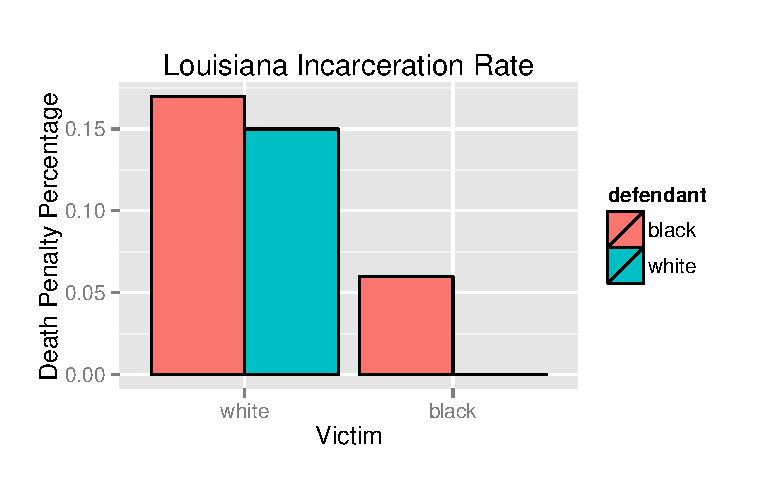
\includegraphics[scale = 0.9]{figures/death_penalty.eps}
    \caption{Death Penalty Summary}
  \end{figure}

\end{document}

